\chapter{Supersimetría y su fenomenología} %%Contexto Te\'orico}

\todo{Add chapter introduction}



%%

% Motivacion (From arxiv 9709356: A susy primer Introduction)
%% The SM of high energy physics, augmneted by neutrino masses, provides a remarkably succesful description of presently known phenomena. The experimental frontier has advance into the
%% TeV range with no uambiguous hints of additinal structure. Still, it seems clear that the SM is a work in progress and will have to be extended to describe physcis at higher energies. Certainly,
%% a new framework will be required at the reduced Planck scale $M_P =  (8\pi G_\text{Newton})^{-1/2} = 2.4 \times 10^{18} \gev$, where quatum gravitational effects become important. Based only
%% on a proper respect for the power of Nature to surprise us, it seems nearly as obvious that new physcis exists in the 16 order of magnitude in eenrgy between the presently explored territory near the electroweak scale,
%% $M_W$, and the Planck scale. ...

El Modelo Est\'andar de la f\'isica de altas energ\'ias, con el agregado de la masa de los neutrinos,
ha tenido un gran \'exito en la correcta descripci\'on de los fenomenos conocidos.
La frontera experimental ha avanzado hasta la escala del \tev\ sin ninguna pista concreta de una
estructura adicional.
Sin embargo, resulta claro que el Modelo Est\'andar es un trabajo preliminar y va a ha tener que ser
extendido para describir la f\'isica de altas energ\'ias.

No hay dudas respecto a que una nueva teor\'ia va a ser necesaria a la escala reducida de Planck
$M_P =  (8\pi G_\text{Newton})^{-1/2} = 2.4 \times 10^{18} \gev$ , donde los efectos cu\'anticos
gravitacionales son importantes. Es bastante claro que tiene que existir nueva f\'isica en los 16
ordenes de magnitud en energ\'ia entre el territorio explorado cerca de la escala electrod\'ebil y
la escala de Planck.

El s\'olo hecho de que la relaci\'on $M_P/M_W$ es tan grande es una gran pista para la f\'isica m\'as
all\'a del Modelo Est\'andar, por el llamado ``problema de jerarquia''. Esta no es una dificultad
intrinseca del Modelo Est\'andar,  but rather a disturbing sensitivity of the Higgs
potential to new physics in almost any imaginable extension of the Standard Model.

The electrically neutral part del campo de Higgs del Modelo Est\'andar es un escalar complejo $H$ con
un potencial clasico $V=m_H^2 |H|^2 + \lambda|H|^4$.

El ME necesita un valor de expectaci\'on del vacio (VEV) para $H$ en el m\'inimo del potencial no nulo.
Esto ocurre si $\lambda>0$ y $m_H^2<0$, resultando en $\langle H \rangle = \sqrt{-m_H^2/2\lambda}$.
Como experimentalmente sabemos que $\langle H \rangle$ es aproximadamente 174 \gev, de las medidas
de las propiedades de las interacciones debiles, el valor de  $m_H^2$ debe ser del orden de $-(100 \gev)^2$.

El problema es que $m_H^2$ recibe grandes correcciones cuanticas de los efectos virtuales de cada
particula a la cual se acopla, directa o indirectamente, al campo de Higgs.

Por ejemplo, en la figura 1.1 tenemos una correci\'on a $m_H^2$ del loop que contiene un fermion de
Dirac $f$ con masa $m_f$. Si el campo de Higgs se acopla a $f$ con un termino en el lagrangiano
$-\lambda_f H \bar{f}f$, el diagrama de Feynman en la figura 1.1 lleva a una correci\'on

\begin{equation}
  \Delta m_H^2 = -\frac{|\lambda_f|^2}{8\pi^2} \Lambda^2_\text{UV} + \ldots
\end{equation}

Ac\'a  $\Lambda_\text{UV}$ es \emph{ultraviolet momentum cutoff} usado para regular \emph{the loop integral}.
%%Debe ser interpretado como la energia minima a la cual entra la nueva fisica que altera el comportamiento
%%it should be interpreted as at least the energy scale at which new physics enters to alter the high-energy behavior of the theory.

Los puntos suspensivos representan terminos proporcioanles a $m_f^2$, que crecen a lo sumo logaritmicamente con
$\Lambda_\text{UV}$. Cualquiera de los leptones o quarks del ME puede jugar el rol de $f$. Para quarks la correccion
tiene que ser multiplicada por 3 para tener en cuenta el color.
La correcion mas grande viene de cuando $f$ el quark \emph{top} con $\lambda_f \approx 1$.

El problema es que si $\Lambda_\text{UV}$ es del orden de $M_P$, la correcion a $m_H^2$ es
30 ordenes de magnitud mas grande que el valor necesario de $m_H^2 \sim (100 \gev)^2$.
Este es solo un problema para las correcciones a la masa al cuadrado del boson de Higgs escalar, porque
las correcciones cuanticas a las masas de los fermiones y los bosones de gauge no tienen una sensibilidad
cuadratica directa a $\Lambda_\text{UV}$ como la que estan en la ecuacion 1.2. Sin embargo, los quarks, leptones
y los bosones de gauge electrodebiles $Z^0$, $W^{\pm}$ del ME, todos obitenen masa de $\langle H \rangle$, por lo
tanto el espectro completo de masas del ME es directa o indirectamnte sensible al cutoff Lambda.

\todo{continue ...}

Afortunadamente la cancelacion de todas estas contribuciones a las masas escalares no solo es posible,
sino es unavoidable, si consideramos que existe una simetria que relaciona fermiones y bosones llamada
supersimetria (SUSY).
Una transformacion supersimetrica convierte un estado bosonico en uno fermionico, y viceversa.
El oprador $Q$ que genera estas transformaciones debe ser un spinor anticonmutativo, con

\begin{equation}
  Q \ket{\text{Boson}} = \ket{\text{Fermion}} \quadd \quadd Q \ket{\text{Fermion}} = \ket{\text{Boson}}
\end{equation}

Los espinores son intrinsecamente objectos complejos, por lo tanto el conjugado hermitico de Q es tambien
un generador de la simetria. Debido a que Q y Qdaga son operadores fermionicos, llevan momento angular de spin
1/2, por lo tanto es claro que susy debe ser una simetria espacio-temporal.



\section{El Modelo Estandar Supersimetrico Minimo (MSSM)} %%The Minimal Supersymmetric Standard Model

\section{Origen del rompimeinto de supersimetria}





%% \begin{figure}[h]
%%   \includegraphics[width=0.8\textwidth]{figures/higgs_loop_correction}
%%   \caption{One-loop quantum corrections to the Higgs squared mass parameter mH2, due to (a) a Dirac fermion $f$, and (b) a scalar S.
%% \end{figure}


%% \begin{fmfgraph}(40,40)
%%   \fmfleft{i}
%%   \fmfright{o}
%%   \fmf{phantom,tension=5}{i,v1}
%%   \fmf{phantom,tension=5}{v2,o}
%%   \fmf{fermion,left,tension=0.4}{v1,v2,v1}
%%   \fmf{photon}{v1,v2}
%% \end{fmfgraph}

\section{Supersimetr\'ia}

Supersimetría (SUSY) \cite{Miyazawa:1966,Ramond:1971gb,Golfand:1971iw,Neveu:1971rx,Neveu:1971iv,%
  Gervais:1971ji,Volkov:1973ix,Wess:1973kz,Wess:1974tw}
es uno de los candidatos teoricos mejores motivados para fisica mas alla del Modelo Estandar.
Si las particulas supersimetricas que interactuan fuertemente, es decir squarks y gluinos, estan
presentes a la scala del \tev, estas deberian haber sido producidas en el LHC incluso a 7 \tev.

Las teorias Gauge Mediated Symmetry Breaking (GMSB) \cite{Dine:1981gu,AlvarezGaume:1981wy,%
  Nappi:1982hm,Dine:1993yw, Dine:1994vc,Dine:1995ag}
consideran un sector oculto en el cual la supersimetria esta rota y la rotura de la simetria
es comunicada a los sectores visibles a traves de las interacciones de bosones de gauge del
modelo estandard.
Estan teorias son especialmente atractivas

Theories of Gauge Mediated Symmetry Breaking (GMSB)  presume a hidden sector in which supersymmetry is
broken and the symmetry breaking is communicated to the visible sectors through Standard Model gauge boson
interactions. Such theories are especially attractive because the hypothesis of an intermediate hidden sector
suppresses the magnitude of flavor-changing neutral currents. The lightest supersymmetric particle (LSP) in GMSB
is the ultra-light gravitino (\gravino), which under certain circumstances is a viable dark matter candidate \cite{Goldberg:1983nd,Ellis:1983ew}.
The \gravino\ has a derivative coupling to each particle and its superpartner with an interaction strength inversely
proportional to $\sqrt{F}$, where $F$  is a vacuum expectation value of an auxiliary field which determines the
magnitude of supersymmetry breaking in the vacuum state.

The phenomenology of GMSB models is determined by the nature of the next-to-lightest supersymmetric particle (NLSP), which for a
large part of the GMSB parameter space is the lightest neutralino \ninoone.

Neutralinos are mixtures of gaugino ($\tilde{B}$, $\tilde{W}^{0}$) and higgsino ($\tilde{H}^{0}_{u},\tilde{H}^{0}_{d}$) eigenstates, and therefore
the lightest neutralino decays to a \gravino\ and either a \gam, Z, or h. If the \ninoone\ is bino-like, the main decay mode is $\ninoone\to\gam\gravino$. If the \ninoone\ is
higgsino-like, it decays as $\ninoone\to h\gravino$. In addition, since the longitudinal polarisation component of the Z boson is also a Goldstone
mode of the Higgs field, a higgsino-like neutralino can also decay as $\ninoone\to Z\gravino$. Consequently, a \ninoone\ pair produced in a collider
can give rise to the diboson final states (hh, h\gam, hZ, Z\gam, ZZ, \gam\gam) + \etmiss. Several searches for these signatures have been performed at the
Tevatron \cite{Abazov:2007ag,Buescher:2005he} and the LHC \cite{Aad:2012zza,Aad:2012jva,Aad:2011kz,Aad2012519,leptonphoton7,Chatrchyan:2011wc,Chatrchyan:2011ah,tagkey2015503}. The scenarios considered in this analysis are the
ones with only one \gam\ %i.e. $\g Z$ and $\g h$,
plus two \gravino\ in the final state, in the case \ninoone\ is a bino-higgsino admixture (\Fig \ref{fig:GGM_diagrams} (left)). Further details on the signal models and benchmark points
considered in this study are given in \Sec \ref{sec:sig_samples}.

In recent years, the effort to formulate GMSB in a model-independent way has led to the development
of general gauge mediation (GGM) \cite{Meade:2008wd,Buican:2008ws}. GGM includes an observable sector with all the MSSM fields,
together with a hidden sector that contains the source of SUSY breaking. In GGM, there need not be any
hierarchy between colored and uncolored states, and therefore there is no theoretical constraint on the
colored-states mass, thus raising the feasibility of GGM discovery even with early LHC data.

This work describes the search for events with an isolated high-\pt\ photon, jets and large \etmiss, in the full dataset of pp collisions
at $\sqrt{s}=8\tev$ recorded in 2012 with the ATLAS detector at the LHC, corresponding to a total integrated luminosity of 20.3 \ifb.
This signature is complementary to other ATLAS searches in \gam\gam+\etmiss \cite{Aad2012519,ATLAS-CONF-2014-001}, $\gam+e/\mu+\etmiss$ \cite{ATLAS-CONF-2012-144}, $\gam+b+\etmiss$ \cite{Aad:2012jva},
and $Z+\etmiss$ \cite{ATLAS-CONF-2012-152} final states. CMS has also performed a similar search \cite{CMS-PAS-SUS-12-018,CMS-PAS-SUS-14-004}, although in the case of a pure bino or wino \ninoone\
state.

%\tosolve{Add experimental searches cites.}
%\tosolve{Comment on CMS measurement?}

\begin{figure}[h!]
  \centering
  \includegraphics[width=0.31\textwidth]{figures/gogo-qqqqphZGG-GMSB}
  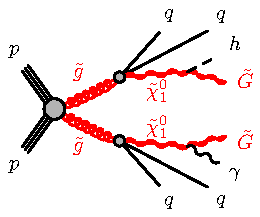
\includegraphics[width=0.31\textwidth]{figures/gogo-qqqqhphGG-GMSB}
  \includegraphics[width=0.31\textwidth]{figures/gogo-qqqqphphGG-GMSB}
  \caption{General production diagrams for GGM photon final states.}
  \label{fig:GGM_diagrams}
\end{figure}

%The next-to-lightest supersymmetric particle (NLSP)
%%defines the phenomenology of these models, and
% is almost always the lightest neutralino \ninoone, often assumed to be a bino-like particle. The bino is the supersymmetric
% partner of the U(1) gauge �eld, coupling to the photon and Z boson with strengths that are determined by the Weinberg
% mixing angle. This results in the \ninoone decaying predominantly to the LSP and a photon. Assuming that R-parity \cite{} is
% conserved, the classical signature of GMSB is, therefore, events with two energetic isolated photons and large missing
% transverse momentum (\etmiss). Searches for such a signature at the LHC and the Tevatron established strong
% experimental constraints on GMSB models \cite{}.

The present analysis is motivated by the bino-higgsino admixture neutralino decay signatures predicted by General Gauge Mediation (GGM) models,
namely a final-state signature that consists of a photon, jets, and high \MET. The event selection described in \Sec \ref{sec:event_selection},
has been designed to maximize the sensitivity to a small signal with this general topology. Any imposition of model-tailored selection cuts has been
avoided, trying to keep the analysis as model independent as possible. However, an interpretation in the framework of a specific model is unavoidable.
A grid of GGM signal points is simulated with a specific set of benchmark parameter values that covers the region in which signal can be established.
The sensitivity of the analysis is evaluated using this grid of points.

In this particular region of the GGM model space, the lightest neutralino is a mixture of bino and higgsino. The neutral wino is much heavier so it
does not contribute. Due to the Weinberg mixing angle in the Standard Model, the bino component of the lightest neutralino couples to both the photon and the Z.
The gluino is regarded as the only relevant coloured sparticle in order to set a conservative limit on the gluino mass. All squark soft masses are set to 2.5 TeV.
The other model parameters are set to M$_2$=2.5 \tev, $\tan\beta$=1.5 and $c\tau_{\mathrm{NLSP}} < 0.1$ mm. The latter assures the neutralino is decaying promptly
and is achieved by making the gravitino sufficiently light ($m_{\tilde{G}}=10^{-9}$ \gev). All trilinear coupling terms are set to zero and masses of sleptons
are set to 2.5 \tev. The Higgs boson is in the decoupling regime with $m_{A}$ = 2 \tev~ and $m_{h}$ = 126 \gev. The last follows the recently measured value
for the SM Higgs boson at the LHC \cite{ATLAS-CONF-2013-014,CMS-PAS-HIG-14-009}. In gauge mediated SUSY scenarios several mechanisms exist \cite{Craig:2011yk,Auzzi:2011eu,Csaki:2012fh,Larsen:2012rq,Craig:2012hc}
to generate a Higgs boson mass as high as this observed value, without changing the phenomenology of the models here considered. No significant effect on the mass spectrum
has been indeed observed when varying this value within a $\pm 10~$ \gev\ range.

\Mone\ and $\mu$ determine the lightest neutralino mass, and are related in such a way that the branching ratios of the \ninoone\ are approximately constant,
resulting in ${\rm BR}(\ninoone \to \gam + \gravino) \approx 50\%$, ${\rm BR}(\ninoone \to Z + \gravino) \approx 49\%$ and ${\rm BR}(\ninoone \to h + \gravino) \approx 1\%$,
numbers which vary by $\pm 1\%$ throughout most of the grid (\Fig \ref{fig:br_n1_x_grav}). For light neutralinos ($<200\gev$) the Higgs production is highly
suppressed and ${\rm BR}(\ninoone \to \gam + \gravino)$ starts falling up to 40\%. The value of $\mu$ must also be positive in order to disfavor the branching ratio
to the Higgs boson, which would lead to a signature already covered by a dedicated analysis in ATLAS \cite{Aad:2012jva}. Similarly, the branching ratio for
($\ninoone \to \gam + \gravino$) is such that maximizes the single photon final state. At larger values the diphoton topology starts to be favoured, which has been
extensively searched for in the past \cite{Aad2012519,Aad:2011kz}. This leaves $M_3$ and $\mu$ as the only two free parameters of the model, spanning the space
within $150\gev < m_{\ninoone} < 1250 \gev$ and $800\gev < m_{\gluino} < 1300 \gev$, with $m_{\ninoone} < m_{\gluino}$. The granularity of the simulation in each
dimension is shown in \Tab\ \ref{tab:signal_pars}, with the resulting value for the gluino and neutralino masses.

The full mass spectrum, the gluino and neutralino branching ratios and decay widths are calculated from
these set of parameters using SUSPECT v2.41 \cite{Djouadi2007426}, SDECAY v1.3b \cite{Muhlleitner:2004mka}
and HDECAY v3.4 \cite{Djouadi:1997yw}, run as part of the SUSYHIT package v1.3 \cite{Djouadi:2006bz}.
An example of the mass spectrum in the configuration is shown in \Fig \ref{fig:mass_spectra}, for one of
the signal grid points. The total decay branching ratios for \gluino-initiated \ninoone\ production are
shown in \Fig \ref{fig:br_gl_n1}, for 2-body\footnote{only effectively, the gluino decays through a virtual
quark-squark loop in this case.} and 3-body gluino decays.
Simulated events were generated with HERWIG++ v2.5.2 \cite{Bahr:2008pv} for the 124 signal points in the
grid (5K per each), using the CTEQ6L1 \cite{Nadolsky:2008zw} parton density distributions. A generator level
filter requiring a photon with $p_{T}>100~$ \gev\ was applied to get higher statistics, specially at low neutralino
mass. The filter efficiency for all simulated points are shown in \Tab \ref{tab:signal_filter_eff}.

Signal production cross sections and uncertainties were calculated using the SUSYSignalUncertainties package \cite{SUSYsigunc}. Cross sections
for the signal processes involving the production of gluino pairs are calculated to next-to-leading order (NLO)
in the strong coupling constant, adding the resummation of soft gluon emission at next-to-leading-logarithmic
accuracy (NLO+NLL) \cite{Beenakker:1996ch,Kulesza:2008jb,Kulesza:2009kq,Beenakker:2009ha,Beenakker:2011fu}.
The EWK $\tilde{\chi}\tilde{\chi}$ production cross sections are calculated to next-to-leading order in the strong coupling constant (NLO) using PROSPINO v2.1~\cite{Beenakker:1999xh}.
%are computed at NLO with Prospino v2.1 \cite{Beenakker:1996ed}.
The cross sections and uncertainties are tabulated in \Tab \ref{tab:signal_xs_strong} and \ref{tab:signal_xs_ewk}, and shown in \Fig \ref{fig:signal_xs_strong} and \ref{fig:signal_xs_ewk}, for the strong and EWK production respectively.
The total nominal cross section and the relative contribution of EWK produced processes are also shown in \Fig \ref{fig:signal_xs_total}.
The total uncertainty is taken from an envelope of cross section predictions using different PDF sets and factorisation and renormalisation scales, as described in \Ref \cite{Kramer:2012bx}. More details of the uncertainties treatment are given in \Sec \ref{sec:syst_signal}. %The dependence of the cross section with $M_3$ is also shown in Fig. \ref{fig:signal_xs}.

All signal samples have been simulated with the faster, parametrized detector simulation ATLFAST-II \cite{Richter-Was:683751}. Derived datasets in the {\sc NTUP\_SUSY}
format are used throughout this analysis, with the configuration tag p1328.








%%%----

%-----------------------------------------------------------------------------------
\section{Gauge-mediated Supersymmetry phenomenology}
\label{sec:susy}
%-----------------------------------------------------------------------------------
Supersymmetry~(SUSY)~\cite{Miyazawa:1966,Ramond:1971gb,Golfand:1971iw,Neveu:1971rx,Neveu:1971iv,Gervais:1971ji,Volkov:1973ix,Wess:1973kz,Wess:1974tw}
introduces a symmetry between fermions and bosons, resulting in a SUSY
partner (sparticle) with identical quantum numbers except a difference
by half a unit of spin for each SM particle. As none
of these sparticles have been observed, SUSY must be a broken symmetry
if realised in nature.  Assuming $R$-parity
conservation~\cite{Fayet:1976et,Fayet:1977yc,Farrar:1978xj,Fayet:1979sa,Dimopoulos:1981zb},
sparticles are
produced in pairs.  These would then decay through cascades involving
other sparticles until the stable, weakly-interacting LSP is produced, leading
to a final state with significant \MET.

Experimental signatures of gauge-mediated SUSY breaking
models~\cite{Dine:1981gu,AlvarezGaume:1981wy,Nappi:1982hm,Dine:1993yw, Dine:1994vc,Dine:1995ag}
are largely determined by the nature of the NLSP.
%In generalized scenarios of gauge-mediated SUSY-breaking
For GGM,
the NLSP can be formed from an admixture of any of the SUSY partners
of the gauge boson and Higgs states.
In this study, three cases are assumed for the
composition of the NLSP. For the first case, the NLSP is assumed to be
purely bino-like (the SUSY partner of the SM U(1) gauge boson). For the
second case, the NLSP is assumed to be an admixture
of the bino and a higgsino that is assumed to be the SUSY partner
of the SM Higgs boson $h$. For the final
case, the NLSP is assumed to be a degenerate triplet
of wino states (the SUSY partners of the SM SU(2) gauge bosons).
In this paper, the neutral NLSP is denoted $\neutralino$ irrespective
of its composition. For the case that
the NLSP is a degenerate triplet, the charged NLSP states are denoted $\chargino$.

For the case that the NLSP is a bino,
the final decay in each of the two cascades in a GGM event would predominantly be
$\neutralino\to\gamma+\gravitino$, leading
to final states with $\gamma\gamma+\met$.
For the case that the NLSP is a mixture of the bino
and higgsino, both the possibilities that the higgsino mass
parameter $\mu$ is less than or greater than zero are explored.
In the former case, the final decay in the cascade would include
a significant contribution from $\neutralino\to h + \gravitino$
with the subsequent decay $h \to \bbbar$, leading to final
states with a photon, multiple $b$-jets, and $\met$.
%(here `$h$' is assumed to have the couplings and branching fractions
%equal to those expected for the SM Higgs boson).
The latter case can produce scenarios for which the
final decay in the cascade can be relatively evenly split
between $\neutralino\to\gamma+\gravitino$ and
$\neutralino\to Z + \gravitino$, leading to final states with
a photon, multiple jets (including two from the hadronic decay of the $Z$ boson)
that typically do not arise from $b$ quarks,
and $\met$.
For the case that the NLSP is a degenerate set of three wino states,
the final step in the cascade includes both charged and neutral wino decays.
Charged wino decays tend to produce isolated
leptons, while neutral wino decays produce photons with a wino-to-photon
branching fraction that is no less than $\sin^2 \theta_W$ for any value of
the wino mass. Overall, these two wino-NLSP contributions lead to a significant
number of events with an isolated photon accompanied by an isolated lepton.
Of the five %seven
GGM models considered here, two (the `gluino-bino' and `wino-bino' models) %three
incorporate a purely bino-like NLSP, two (the `higgsino-bino' models)    %three
incorporate an NLSP that is a higgsino-bino admixture, and one (the `wino-NLSP' model)
incorporates a wino-like set of NLSPs; in all cases
the mass of the NLSP state is considered to be a free parameter
of the model.
A summary of these models,
including their motivating experimental signatures, is presented in Table~\ref{tab:GGM_models}.

\begin{table}[bp]
  \caption{Summary of the five GGM models considered in this study. For the two higgsino-bino
models, the functions $f_{\pm}(M_1,\mu)$ are chosen to establish NLSP decay properties
commensurate with the target experimental signature, as described in the text.}
  \begin{center}
  \begin{tabular*}{\textwidth}{@{\extracolsep{\fill}}lrrrr} \hline
                            & Experimental       & Produced        & Composition    &  Free                \\
    {\bf GGM Model}         & Signature          & State(s)        & of NLSP        &  Parameters          \\
      \noalign{\smallskip}\hline\noalign{\smallskip}
    Gluino-bino             & diphoton           & gluino           & bino          & $M_{\gluino}$,$M_{\neutralino}$ \\
    Wino-bino               & diphoton           & wino             & bino          & $M_{\wino}$,$M_{\neutralino}$   \\
    Higgsino-bino ($\mu<0$) & photon+b           & gluino, higgsino & higgsino/bino & $M_{\gluino}$,$f_{-}(M_1,\mu)$          \\
    Higgsino-bino ($\mu>0$) & photon+j           & gluino, higgsino & higgsino/bino & $M_{\gluino}$,$f_{+}(M_1,\mu)$          \\
    Wino NLSP               & photon+$\ell$      & wino             & wino          & $M_{\wino}$          \\
      \noalign{\smallskip}\hline\noalign{\smallskip}
  \end{tabular*}
  \label{tab:GGM_models}
  \end{center}
\end{table}


The two %three
GGM models incorporating a bino-like NLSP
are the focus of the diphoton analysis. For these models,
one other set of SUSY partner states is taken to be potentially
accessible in 8 TeV {\it pp} collisions, while
all other SUSY mass parameters are decoupled (set to
inaccessibly large values). For both %all three
of these bino-like NLSP cases, production
proceeds solely through this set of SUSY partners,
with the NLSP appearing in the subsequent
decays of the produced SUSY partner states. For the gluino-bino
model, the set of partners is composed of a degenerate octet of
gluinos (gluon partners).
%Also considered is a `squark-bino' model for which production proceeds through a mass-degenerate
%set of squarks (quark partners),
%including all
%squark flavors and chiralities of squarks excepting
%the right-handed up-type squark,
%whose mass is decoupled.
For the `wino-bino' model, the set of partners is composed
of a degenerate triplet of wino states
\neutralinotwo, \chargino, and is dominated by the production
of \chiplus\chiminus and \neutralinotwo\chargino.
For both %all three
of these models, the masses of these produced states
are considered to be free parameters along with that of the chosen
\neutralino state, the latter of which is constrained to be less
than those of the produced states.
This results in a SUSY production
process that proceeds through the creation of pairs of the higher-mass
states, which subsequently decay through
short cascades to the NLSP \neutralino states. Other SM
objects (jets, leptons, photons) may be produced in these cascades.
The \neutralino branching fraction
to $\gamma$ + \gravitino is 100\% for $m_{\neutralino} \to 0$ and
approaches $\cos^2 \theta_W$ for $m_{\neutralino} \gg m_Z$, with
the remainder of the \neutralino sample decaying to $Z$ + \gravitino.
For all \neutralino masses, then, the branching fraction is dominated
by the photonic decay, leading to the diphoton-plus-\met signature.
For these models with a bino-like NLSP, typical production and decay channels for strong (gluino) and
electroweak (wino) production are exhibited in Fig.~\ref{fig:feynman_bino}.

\begin{figure}[tp]
  \begin{center}
    \includegraphics[width=0.45\textwidth]{gogo-qqqqphphGG-GMSB} ~~
    \includegraphics[width=0.45\textwidth]{C1C1-WWphphGG-GGM}
  \end{center}
  \caption{
Typical production and decay-chain processes for the gluino-production (left)
      and electroweak-production (right) instances of the
      GGM model for which the NLSP is a bino-like neutralino.
%      For the higgsino-bino models, the final
%      step of the cascade (the \neutralino decay) would have a
%      probability of order 50\% for producing a Higgs
%      (for the model with $\mu < 0$) or $Z$ (for the model with $\mu > 0$)
%      boson.
    \label{fig:feynman_bino}
  }
\end{figure}

\begin{figure}[tp]
  \begin{center}
    \includegraphics[width=0.45\textwidth]{gogo-qqqqbbphGG-h} ~~
    \includegraphics[width=0.45\textwidth]{gogo-qqqqphZGG-GMSB}
  \end{center}
  \caption{
    Typical production and decay-chain processes for the gluino-production
    and electroweak-production instances of the
    GGM model for which the NLSP is a higgsino-bino neutralino admixture.
    For the model with $\mu < 0$ (left), the final
    step of the cascade (the \neutralino decay) would have a
    probability of order 50\% of producing a Higgs boson rather than a
    photon or $Z$ boson; for the model
    with $\mu > 0$ (right), the \neutralino decay would have a
    probability of order 50\% of producing a Z boson rather than a photon.
    \label{fig:feynman_higgsino_bino}
  }
\end{figure}

\begin{figure}[tp]
  \begin{center}
    \includegraphics[width=0.45\textwidth]{C1N1-phlvGG-W}
  \end{center}
  \caption{
Typical production and decay-chain processes for the wino-NLSP model.
In this model, the \neutralino is a pure \winon state, while the
\chargino are the two charged wino states.
    \label{fig:feynman_wino}
  }
\end{figure}

%Three
The higgsino-bino GGM models incorporate an NLSP composed of
a higgsino-bino admixture, as well as
%including `gluino-higgsino'%, `squark-higgsino'
%and `gluino-higgsino-jets' models that incorporate degenerate sets
a degenerate octet of gluinos %and squarks
identical in nature to those of the
gluino-bino model. % and squark-bino models, respectively.
For the first %two
of these models, which is the focus of the photon+b analysis,
the higgsino mass parameter $\mu$ is required to be negative, and the composition
of the NLSP is set by adjusting $\mu$ and the GGM U(1) mass parameter
$M_1$ so that a constant ratio of the branching fraction of $\neutralino \to h + \gravitino$
to that of $\neutralino \to \gamma + \gravitino$ is maintained at
approximately 1.7:1 over the full range of NLSP masses.
In the limit that $m_{\neutralino} \gg m_Z$, the NLSP
branching fractions to $h + \gravitino$, $\gamma + \gravitino$,
and $Z + \gravitino$ approach 56\%, 33\%, and 11\%, respectively.
The GGM SU(3) mass parameter $M_3$ bears a direct relation to the
gluino mass, and is taken to be a free parameter in this $\mu < 0$ higgsino-bino
model, with all squark states decoupled.
%For the squark-higgsino model, the gluino
%mass and the mass of the right-handed up-type squark are decoupled, with the
%remaining squark masses treated as a single free parameter. For both of these models,
The GGM SU(2) mass parameter $M_2$ is set to a value of 2.5 TeV.
Four other electroweak gaugino states typically lie
within 25 GeV of the \neutralino NLSP: the two lightest charginos \chargino, and two
additional neutralinos \neutralinotwo and \neutralinothree.
The pair production of gluinos or any of these four additional gaugino
states leads to decays to the \neutralino via
cascades involving SM particles.

For the second of the higgsino-bino models, which is
the focus of the photon+j analysis, the $\mu$ parameter is
chosen to be positive, which suppresses the $h + \gravitino$
decay mode of the higgsino. As for the models described above,
the NLSP mass is taken to be a free parameter.
The $M_1$ and $\mu$ parameters are adjusted so that the branching
fractions of the $\neutralino$ to $\gamma + \gravitino$, $Z + \gravitino$
and $h + \gravitino$ are maintained close to 50\%, 49\% and 1\% for
most values of the $\neutralino$ and gluino masses.
In this model, the production of gluino pairs can be followed
by decays to both a single photon and a hadronically-decaying $Z$ boson, producing
events with a single isolated high-energy photon accompanied
by two jets.
In the case that the gluino mass is substantially
larger than the $\neutralino$ mass, additional jets can
be produced in the cascade.
Three additional electroweak gaugino states
lie close in mass to the \neutralino, allowing for the
possibility of SUSY production through pairs of these
states. Such events tend to produce fewer jets than those that proceed through gluino production,
but in certain regions of the model space can provide a significant
contribution to data samples selected to isolate the photon-plus-jets
signature. As for the $\mu < 0$ higgsino-bino model, the value of $M_3$, which is directly
related to the gluino mass, is taken to be a free parameter, $M_2$ is
set to a value of 2.5 TeV, and all squark states are decoupled.
Typical production and decay-chain processes for the two models
for which the NLSP is a higgsino-bino admixture are shown in Fig.~\ref{fig:feynman_higgsino_bino}.


Finally, the wino-NLSP model, which is the focus of the photon+$\ell$ analysis,
incorporates a set of three degenerate wino-like
NLSPs. This set includes the neutral \winon, which as the lightest
neutral gaugino is also referred to as the \neutralino,
as well as the two charged wino states, which form the \chargino states.
Production proceeds
%either through pairs of colored sparticles or
through the direct production of pairs of NLSP states;
%In either case
%the decay procedes through two wino-like NLSPs, and as a result
such events usually contain at least one \winon NLSP. Although
the \winon couples preferentially to the $Z$ boson relative to
the photon, the \winon decays into a photon+gravitino final state with unit branching fraction
for wino mass below that of the $Z$ boson.
The \winon branching fraction to photon+gravitino approaches
$\sin^2 \theta_W$ for wino masses far above that of the $Z$ boson.
Leptons can be produced either through the decays of charged wino
states, or through the decays of $Z$ bosons that arise from \winon
decay, leading to a significant probability that the overall final state
will contain both a photon and a lepton. In this model,
%a common squark and guino mass is taken as a free parameter
%along with the wino NLSP mass scale;
a common wino mass scale is taken as a free parameter, with
all other GGM mass parameters set to a value of \unit[2.5]{TeV}, except the squark masses,
which are set to infinity.
A production and decay diagram typical for this model is shown in Fig.~\ref{fig:feynman_wino}.
%In all cases, the decay chain
%procedes through the wino-like NLSP states.


For all five models considered here, the mass of the gravitino is chosen so that
the NLSP decay length is never greater than 1 mm. This ensures that all
particles arising from the decay of the NLSP are prompt, and in particular that
that the relationship between the point and direction of impact
of photons from NLSP decay upon the face of the detector is
consistent with that of a prompt photon (a separate analysis~\cite{Aad:2014gfa}
searches for GGM models with a longer-lived bino-like NLSP, leading to signatures with non-prompt photons).
In addition, the ratio
$\tan \beta$ of the two SUSY Higgs-doublet vacuum-expectation values is set to a value of 1.5;
%for all but the higgsino-bino model with positive $\mu$ and the wino-NLSP model; for those models
%$\tan \beta$ is set to 1.5.
for all five models, the phenomenology relevant to this search is only
weakly dependent on the value of $\tan \beta$.
